%!TEX root = ../../thesis.tex
%*******************************************************************************
%****************************** Concept Chapter *********************************
%*******************************************************************************

\chapter{Solution Concept}

\ifpdf
    \graphicspath{{Chapters/Solution-Concept/Figs/}{Chapters/Solution-Concept/Figs/}{Chapters/Solution-Concept/Figs/}}
\else
    \graphicspath{{Chapters/Solution-Concept/Figs/}{Chapters/Solution-Concept/Figs/}}
\fi
The Solution Concept chapter in software engineering provides a comprehensive understanding of the proposed solution approach. 
In this chapter, we present the conceptual design of the solution, which outlines the system's key features, components, and functionalities. 
This chapter bridges the gap between the problem statement and the actual implementation of the solution by providing a detailed description of the solution approach. 
It lays the groundwork for the development process, including the design decisions, architectural patterns, and technologies used to build the software implementation. 
Overall, in this chapter, we conceptualize the design based on the LEAN development cycle.

\section{Component Diagram}
\label{sc:section:componentD}
\begin{figure}[htbp!]
    \centering    
    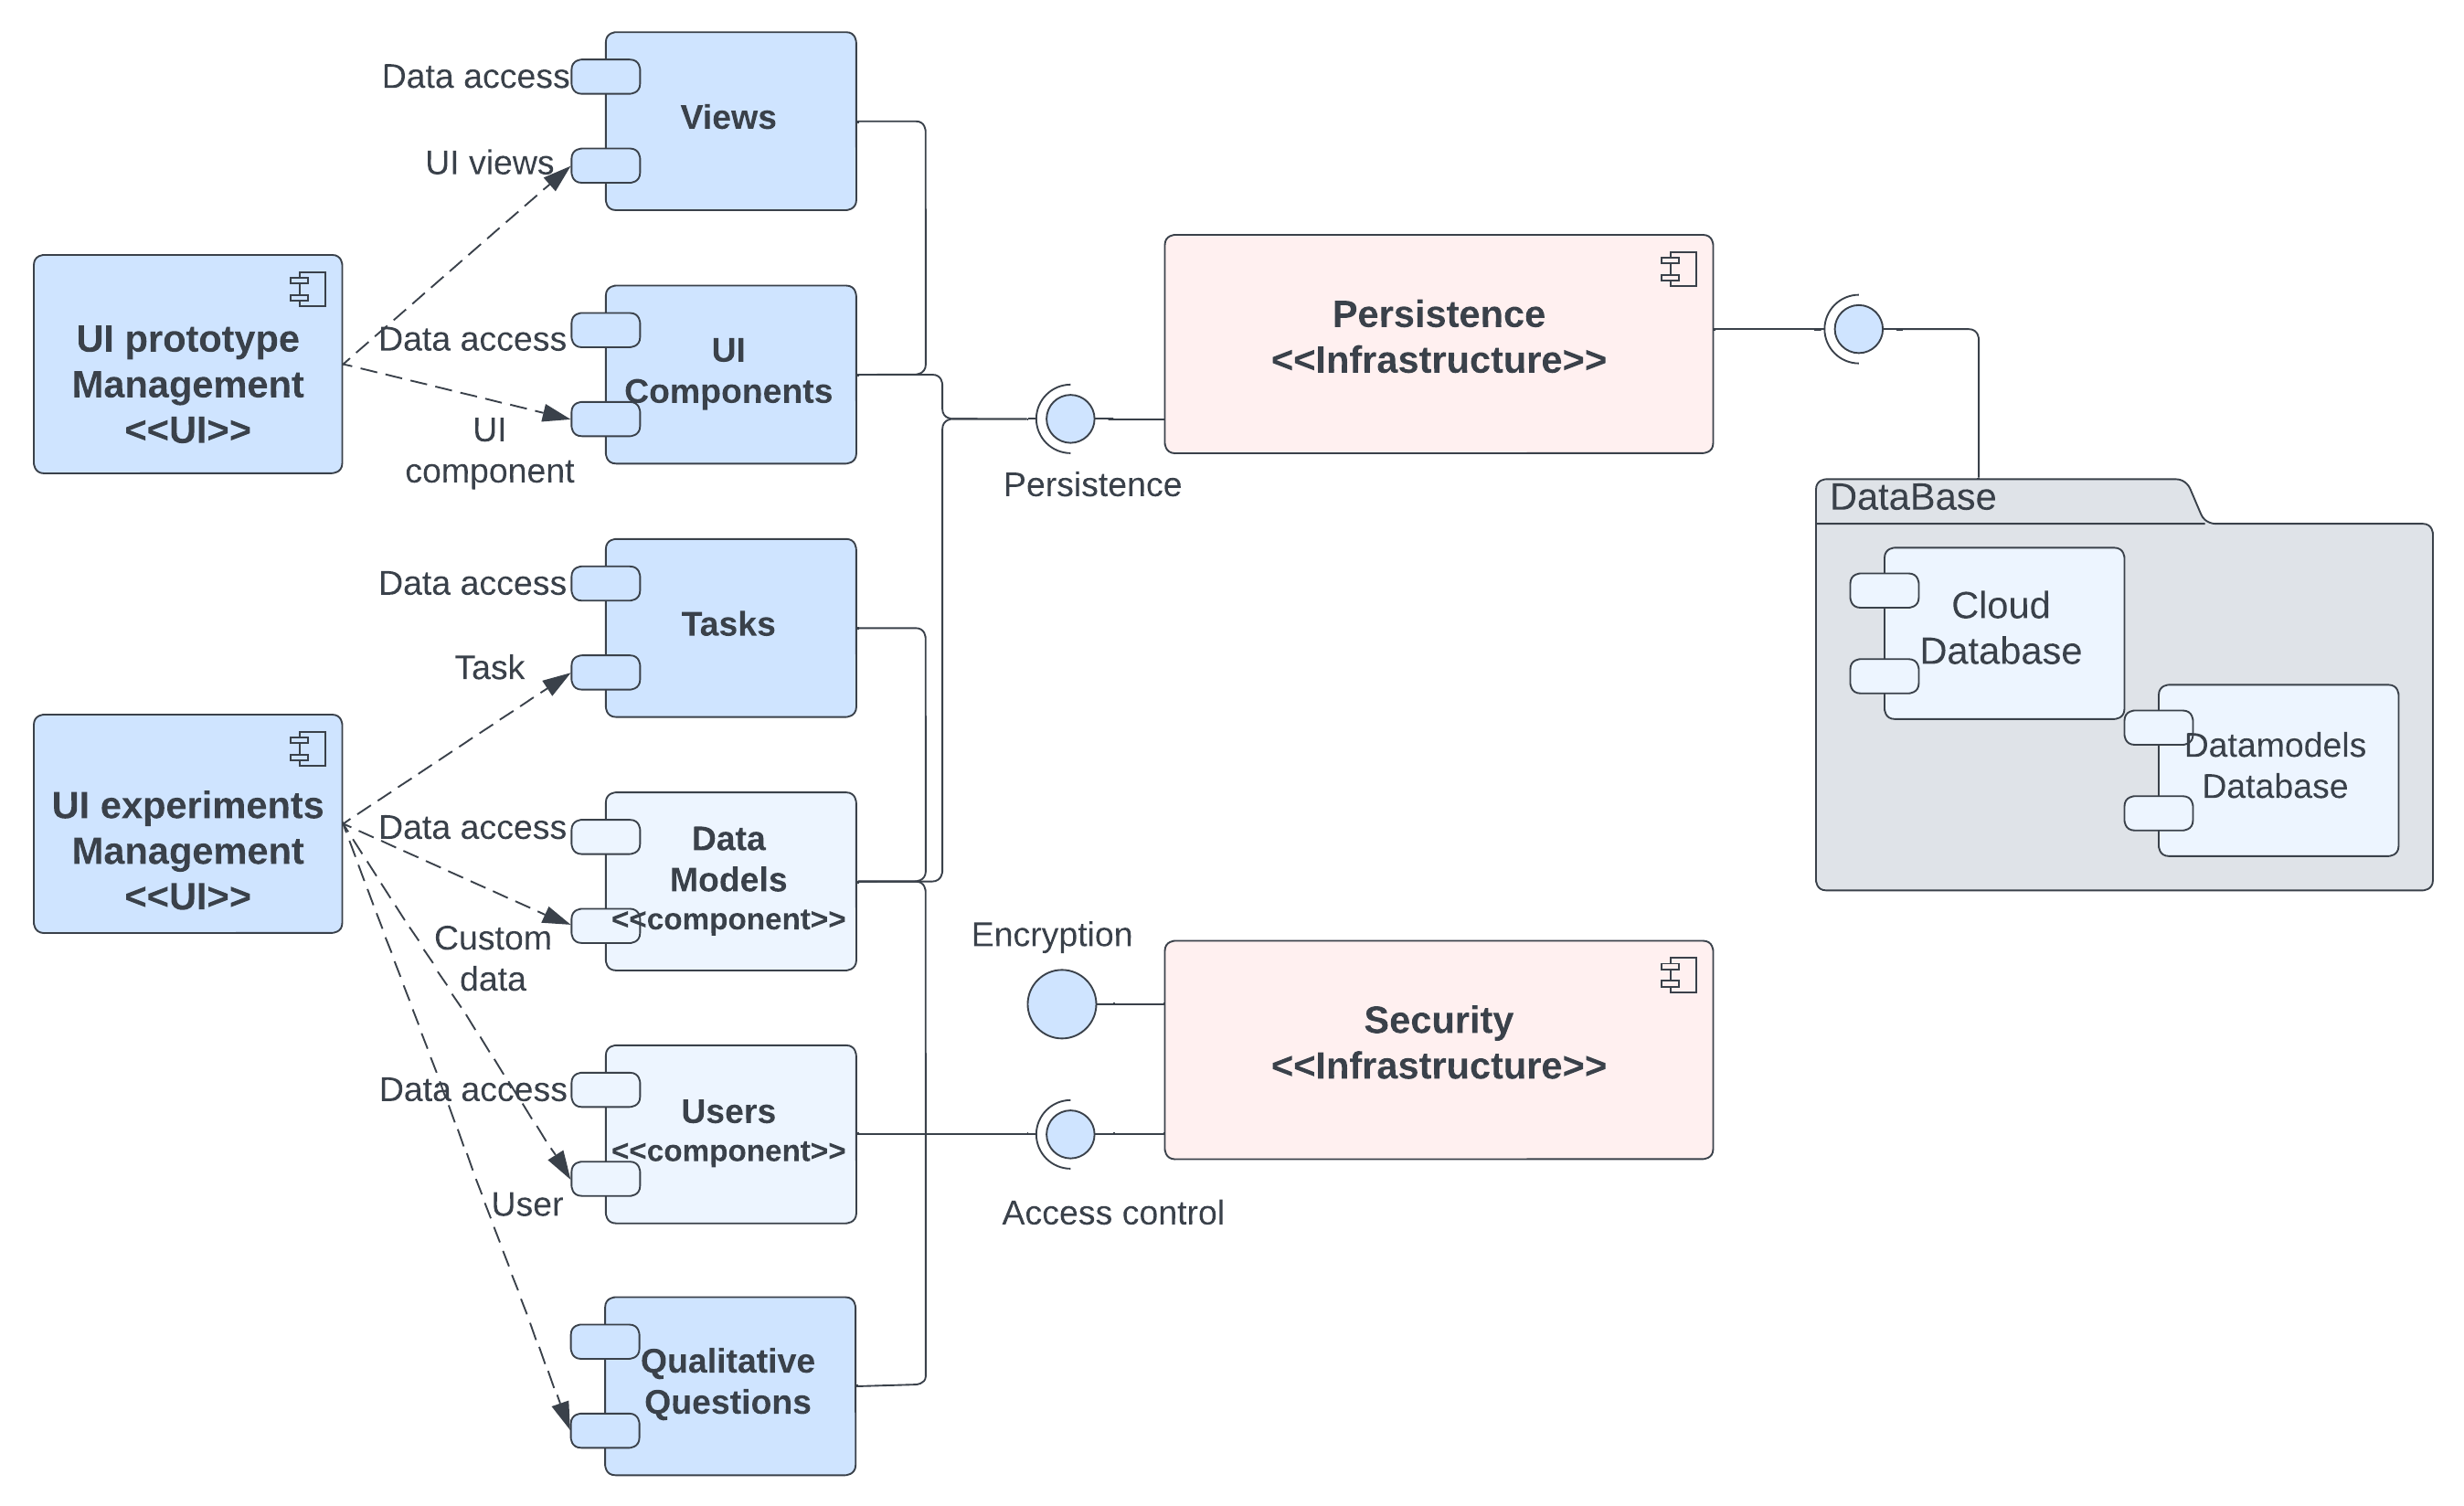
\includegraphics[width=1\textwidth]{Component_d.png}
    \caption[Copmponent Diagram]{Solution Concept for a UI Prototyping tool using LEAN development}
    \label{fig:sc:componentD}
\end{figure}

\section{Code Generation}
\label{sc:section:codeGeneration}

\section{UI Prototyping}
\label{sc:section:prototyping}

\paragraph{Views}

\paragraph{UI Components}

\section{Experimentation}
\label{sc:section:experimentation}

\paragraph{Creating Tasks}

\paragraph{Data Models}

\paragraph{User Management}

\paragraph{Qualitative Questions}